% !TeX root = ../../../main.tex

In the absence of intrinsic charm, the charm \pdf is fully determined by
perturbative matching conditions, i.e.\ by the matrix
$\mathbf{A}^{(n_f)}(Q_{c}^2)$ in Eq.~(\ref{eq:ic/EKO2}).
%
We will denote the
charm \pdf thus obtained
``perturbative charm \pdf'', for short. The \pdf
uncertainty on the perturbative charm \pdf is directly related to that 
of the light quarks and especially the gluon, and is typically much smaller
than  the  uncertainty on our default charm \pdf, that includes
intrinsic charm. Here and in the following we will refer to our final
result, as shown in Fig.~\ref{fig:ic/charm_content_3fns} (right) as ``default''.
%
It should be noticed that the matching conditions for charm are 
nontrivial starting
at \nnlo: at \nlo the perturbative charm \pdf vanishes at threshold.
%
Hence, having implemented in EKO also the \nnnlo matching conditions,
we are able to assess the MHOU of the perturbative charm at the
matching scale $Q_c$, by comparing
results obtained at the first two nonvanishing perturbative
orders.

As already mentioned, see also Fig.~\ref{fig:ic/Zc}~(top left) in the main manuscript, we have
constructed a \pdf set with perturbative charm, in which the full \pdf
determination from the global dataset leading to the NNPDF4.0 \pdf set
is repeated, but now with the assumption of vanishing intrinsic charm,
i.e.\ with a perturbative charm \pdf.
%
This perturbative charm \pdf is compared to our default result
in Fig.~\ref{fig:ic/charm_fitted_vs_perturbative_mhous}~(left), where the 4\fns
perturbative 
charm \pdf at scale  $Q_c=m_c$ obtained using either \nnlo or \nnnlo
under the assumption of no intrinsic charm are shown, together with
our  result allowing for intrinsic charm.
%
It is clear that while on the one hand, the \pdf uncertainty on the
perturbative charm \pdf is indeed tiny, on the other
hand the difference between the result for perturbative charm
obtained using \nnlo or \nnnlo matching is large, and in
fact larger at small $x$ than the difference between perturbative charm and our
default (intrinsic) result.

%%%%%%%%%%%%%%%%%%%%%%%%%%%%%%%%%%%%%%%%%%%%%%%%%%%%%%%%%%%%%%%%%%%%%%%%%%
%%%%%%%%%%%%%%%%%%%%%%%%%%%%%%%%%%%%%%%%%%%%%%%%%%%%%%%%%%%%%%%%%%%%%%%%%%
\begin{figure}[h]
  \begin{center}
    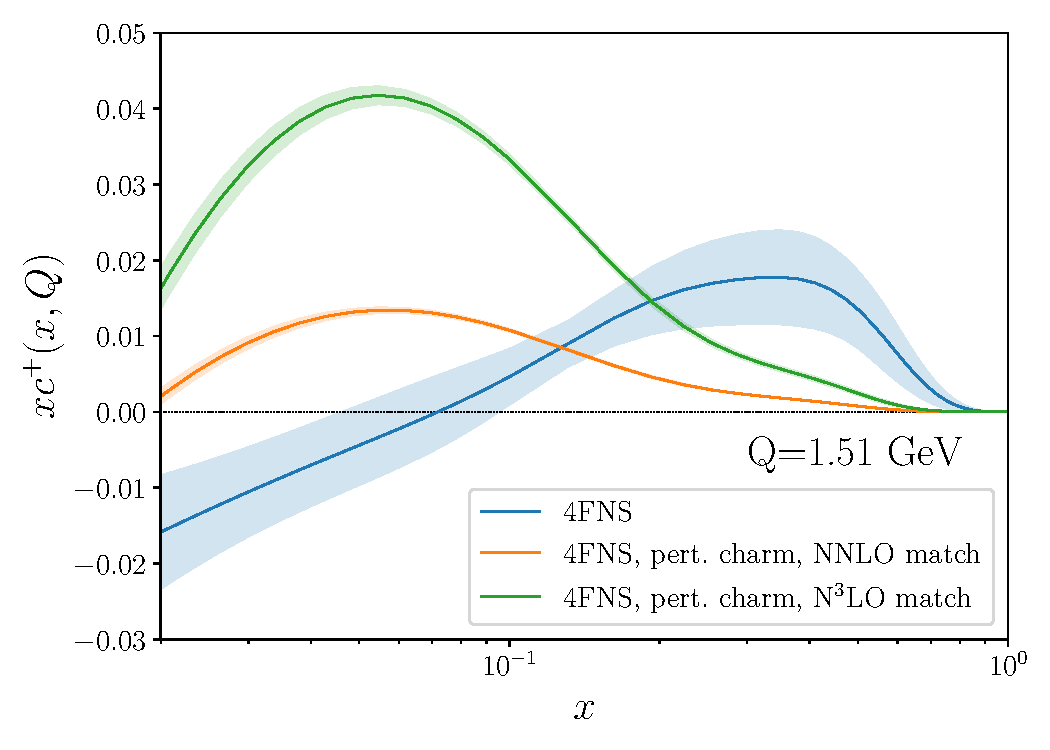
\includegraphics[width=0.49\linewidth]{ch-ic/pch_vs_fitted_forward.pdf}
    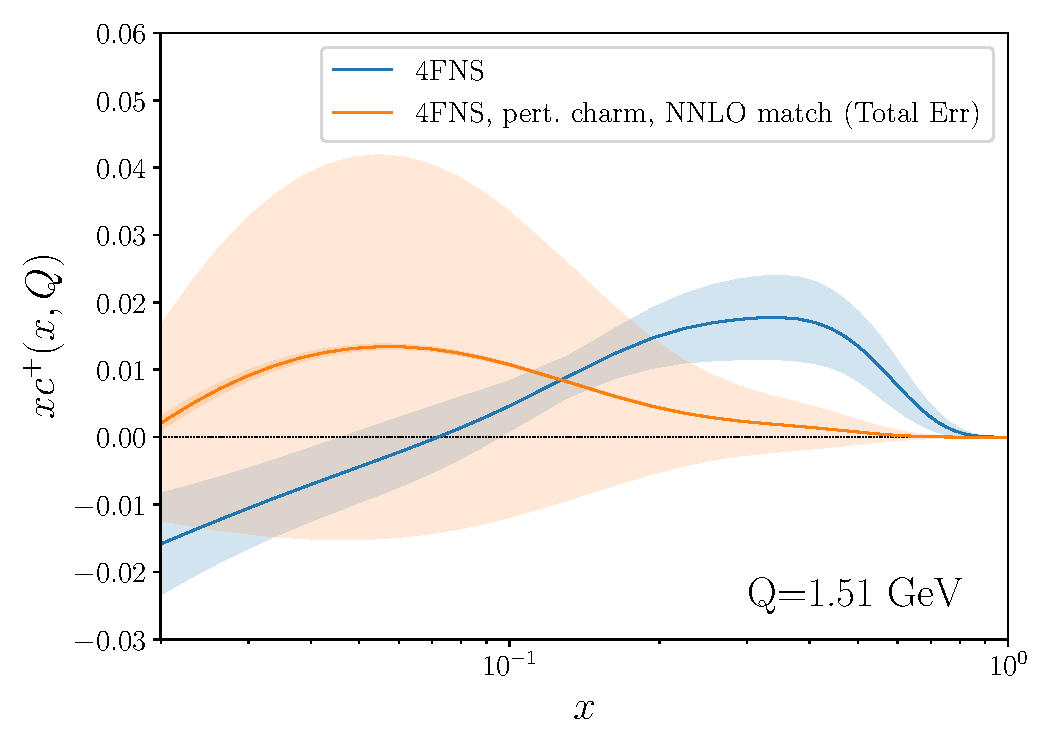
\includegraphics[width=0.49\linewidth]{ch-ic/pch_vs_fitted_forward_MHOU.pdf}
    \caption{\small Left: the perturbative charm \pdf at $Q=1.51$~GeV
  obtained from \nnlo \pdfs using \nnlo and \nnnlo matching
    conditions.
      %
      Right: the \nnlo perturbative charm \pdf including the MHOU
    computed as the difference between \nnlo and \nnnlo matching.
In both plots our default (intrinsic) charm \pdf is also shown for comparison.  
  \label{fig:ic/charm_fitted_vs_perturbative_mhous} }
\end{center}
\end{figure}
%%%%%%%%%%%%%%%%%%%%%%%%%%%%%%%%%%%%%%%%%%%%%%%%%%%%%%%%%%%%%%%%%%%%%%%%
%%%%%%%%%%%%%%%%%%%%%%%%%%%%%%%%%%%%%%%%%%%%%%%%%%%%%%%%%%%%%%%%%%%%%%%%

In the same manner as we used the difference between the results obtained from
inversion of \nnlo and \nnnlo  matching as an estimate of the MHOU on
intrinsic charm, we may use the difference between the 4\fns
 perturbative charm obtained from \nnlo and \nnnlo matching as an
 estimate of the MHOU on perturbative charm at the scale $Q_c$.
 %
 The total uncertainty is found by adding
 this in quadrature to the \pdf uncertainty (which however in practice
 is negligible).
%
The result is shown in 
Fig.~\ref{fig:ic/charm_fitted_vs_perturbative_mhous}~(right).
Within this total uncertainty there is now good agreement between our
intrinsic charm result and perturbative charm for all
$x\lsim 0.2$. On the other hand, there is a clear deviation for larger
$x$. We may view the difference between the 4\fns default result
and the 4\fns perturbative  charm as the intrinsic component in the
4\fns, and indeed it is clear from
Fig.~\ref{fig:ic/charm_fitted_vs_perturbative_mhous} that the 4\fns
intrinsic component is sizable and positive at large $x$.
%
This is of course consistent with our main finding that we
only see evidence of intrinsic charm for large $x\gsim 0.2$, while for
smaller $x$ our result for the charm \pdf is compatible with zero, as demonstrated by
Fig.~\ref{fig:ic/charm_content_3fns}~(right) in the main manuscript.

